\documentclass{article}

\usepackage{color}
\usepackage{enumitem}
\usepackage{graphicx}
\usepackage{amssymb}
\usepackage{hyperref}

%----------------------------------------------------------------------------

\def\d{{\rm d}}
\def\un#1{\,{\rm #1}}
\def\ung#1{\quad[{\rm #1}]}
\def\unt#1{[{\rm #1}]}
\def\e{{\rm e}}
\def\I{{\rm i}}
\def\T{{\rm T}}
\def\vec#1{\mathbf{#1}}
\def\mat#1{\mathsf{#1}}
\def\etal{et al.}
\def\todo#1{{\color{red}TODO: #1}}
\def\TODO#1{{\color{red}TODO: #1}}

\setbox123\hbox{$0$}
\setbox124\hbox{$.$}
\def\S{\hbox to\wd123{\hss}}
\def\.{\hbox to\wd124{\hss}}

\def\Name#1{#1, }
\def\Review#1#2#3#4{{\it #1} {\bf #2} (#3) #4}

\def\hang{\hangindent=\parindent}
\catcode`\>=11
\newskip\itskip \itskip2mm
\newskip\iitskip \iitskip0mm
\newdimen\itindent \itindent3mm
\newdimen\iitindent \iitindent5mm
\def\>{\par\vskip\itskip\parindent\itindent\indent\hang\llap{\hbox to3mm{$\bullet$\hss}}}
\def\>E{\par\vskip\itskip\parindent\itindent\indent\hang\llap{\hbox to3mm{\hss}}}
\def\>>{\par\vskip\iitskip\parindent\iitindent\indent\hang\llap{\hbox to\iitindent{\hss--\ }}}

%----------------------------------------------------------------------------------------------------

\hoffset=0cm
\oddsidemargin=0cm
\textwidth=17cm

%----------------------------------------------------------------------------------------------------

\begin{document}

\centerline{version 1} % sent on 5 Jan 2017
\vskip2cm

%----------------------------------------------------------------------------------------------------

This could be a good reference for TOTEM, its RPs, etc.~\cite{totem-jinst}.

\section{Alignment}
\label{s:alignment}

The alignment proceeds in two stages. In the first stage, the alignment is performed with data from a special low-luminosity calibration fill, where both horizontal and vertical RPs are inserted very close to the beam (about $5\un{\sigma}$). In the second stage, this alignment information is transferred to the standard physics fills with high luminosity and only horizontal RPs inserted.

The first stage employs the standard TOTEM alignment procedure, see e.g.~Section 3.4 in \cite{totem-ijmp}, which includes the following three steps.
\begin{enumerate}[noitemsep]
\item {\em Beam-based alignment} -- a procedure which takes place before data-taking and the purpose of which is to align the RPs with the LHC collimators and the circulating beam. For that collimators scrape the beam to have a sharp edge and then each RP is slowly approached until a contact with the beam is signalised by a spike in beam-loss monitors downstream.
\item {\em Relative alignment among RPs} is achieved by analysing residuals between hits and track fits within each RP station. In this step, position (shift in the read-out direction) and rotation (about the beam axis) of each Si sensor is optimised. Thanks to the overlap between the horizontal and vertical RPs, the relative position among all sensors can be determined. For details see Section 4.2 in \cite{jan_thesis}.
\item {\em Absolute alignment wrt.~the beam} is performed with a sample of elastic-scattering events tagged by the vertical RPs. Due to the azimuthal symmetry of the process, the position of the beam can be derived from the observed hit distributions.
\end{enumerate}

For the second alignment stage, the method relies on the physics being the same both in the calibration and physics fills. Assuming that the LHC settings (optics, collimators, etc.) are the same, too, the hit distribution observed in a physics fill can be aligned/matched to the distribution from the calibration fill. Data used for this matching come from standard CMS triggers which do not use any RP information and are therefore close to zero-bias regarding forward protons. Then, a ``cleaning cut'' is applied in each arm of the spectrometer requiring a correlation between the horizontal hit position in the near and far RP, which is fulfilled by physics tracks originating at the IP. Several metrics of hit-distribution matching have been explored, focusing first on the horizontal alignment essential for $\xi$ reconstruction. An example is shown in Figure \ref{fig:al_matching}, left. The matching procedure has been applied separately to every RP and every fill in order to check for time-dependent effects and control of systematic errors. An example of results is shown in Figure \ref{fig:al_matching}, right. As expected, the difference between results from fills with and without the safety margin is compatible with $0.5\un{mm}$ and within each group the results are compatible with a constant. The uncertainty, dominated by the systematic fill-to-fill differences, is estimated to about $150\un{\mu m}$.

\begin{figure}[h!]
\begin{center}
\hskip-2mm
\raise2.4mm\hbox{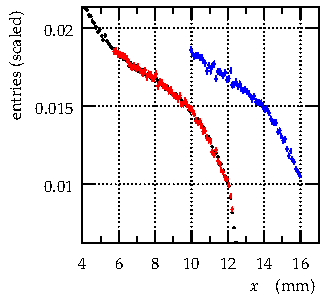
\includegraphics{fig/summary/match_method_example.pdf}}
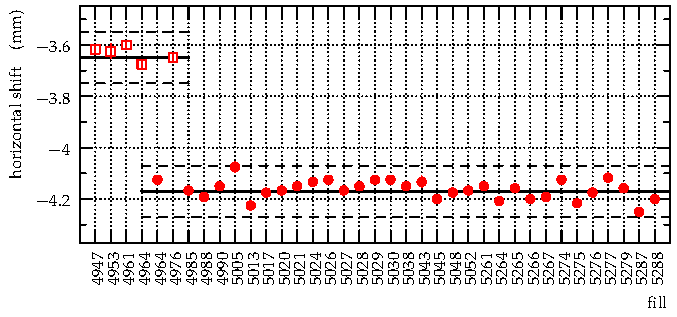
\includegraphics{fig/summary/match_result_cmp_mean.pdf}
\hskip-2mm
\caption{%
{\it Left}: Example of hit distribution matching -- comparison of histograms of horizontal track positions in RP 45-210-fr-hr. The black histogram corresponds to the calibration fill (TOTEM run 10081), the blue (red) histograms to a physics fill 4964 before (after) the matching.\hfil\break
{\it Right}: Summary of horizontal corrections obtained by the matching procedure for RP 45-210-fr-hr in each fill. The fills with and without the safety margin are represented by hollow squares and filled circles, respectively. The error bars indicate statistical uncertainties only. The continuous black lines show constant fits through each fill group, the dashed black lines show the final uncertainty estimate.
}
\label{fig:al_matching}
\end{center}
\end{figure}



%----------------------------------------------------------------------------------------------------

\section{Optics determination}
\label{s:optics}


%----------------------------------------------------------------------------------------------------

\section{Alignment and optics validation}
\label{s:validataion}

This section presents a simple validation of the alignment and optics calibration, based on the fact that the four RPs, in all fills, measure the same physics, up to the detector effects (acceptance, resolution, etc.). As a reference physics quantity, inclusive $\xi$ spectra will be used after the ``cleaning cut'' introduced in Section \ref{s:alignment}.

\TODO{Not mentioning how $\xi$ reconstructed since it presumably is already at a different place of the article.}

Figure \ref{fig:al_opt_val}, left, shows an event-by-event correlation of $\xi$ values reconstructed in the near and far RP of the left spectrometer arm. As expected, the correlation is very close to the dashed line representing equality of both $\xi$'s.

Figure \ref{fig:al_opt_val}, middle, compares the $\xi$ distributions from several fills but the same RP. Apart from the lower-$\xi$ regions affected by the radiation damage, there is a very good overlap with the thick black histogram originating from the calibration run. This manifests the stability of the calibration procedures.

Figure \ref{fig:al_opt_val}, right, compares the $\xi$ distributions from the same fill but different RPs. Disregarding the region $\xi\gtrsim 0.08$ affected by acceptance limitations, one can observe a good shape agreement among the histograms from all the four RPs.


\begin{figure}[h!]
\begin{center}
\hskip-15mm
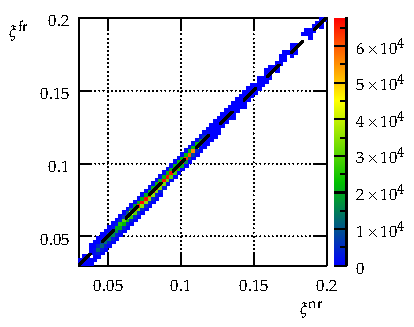
\includegraphics{fig/summary/xi_NF_corr_cmp.pdf}
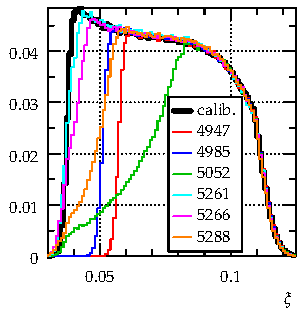
\includegraphics{fig/summary/xi_cmp_run.pdf}
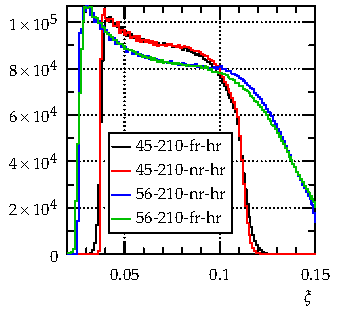
\includegraphics{fig/summary/xi_cmp_rp.pdf}
\hskip-15mm
\caption{%
{\it Left}: Correlation of $\xi$ values determined from 45-210-fr-hr (vertical axis) and 45-210-nr-hr (horizontal axis), data from fill 5026. The dashed black line indicates the line where both $\xi$'s are equal.
\hfil\break
{\it Middle}: Comparison of $\xi$ distributions determined from 45-210-fr-hr and different fills, see legend. The reduced efficiency/acceptance at the low-$\xi$ end is due to radiation damage of the sensors.
\hfil\break
{\it Right}: Comparison of $\xi$ distributions determined by different RPs in the calibration fill (TOTEM run 10077).
}
\label{fig:al_opt_val}
\end{center}
\end{figure}



%----------------------------------------------------------------------------------------------------

\begin{thebibliography}{99}

\bibitem{totem-jinst}
	\Name{G.~Anelli \etal{}~(TOTEM Collaboration)}
	\Review{JINST}{3}{2008}{S08007}.
    %The TOTEM Experiment at the CERN Large Hadron Collider, JINST 3 S08007, 2008

\bibitem{totem-ijmp}
	\Name{G.~Antchev \etal{}~(TOTEM Collaboration)}
	\Review{Int.~J.~Mod.~Phys.~A}{28}{2013}{1330046}.

\bibitem{jan_thesis}
	\Name{J.~Ka\v spar}
	PhD Thesis, CERN-THESIS-2011-214,
	\url{http://cdsweb.cern.ch/record/1441140}.

\end{thebibliography}

\end{document}
